%----------------------------------------------------------------
% Preamble
%----------------------------------------------------------------
\documentclass[12pt, aspectratio=169, xcolor=dvipsnames]{beamer} 			         % Document class
% \documentclass[12pt, aspectratio=169,xcolor=dvipsnames,handout,notes=show]{beamer}	  % For printing
\input{../Settings/packs_beamer}   		  % Packages
%% Personalized Macros
% Definitions, Equations, Table of Contents, Tables, Subcaptions, Paths, Text Fomats

%-------------------------------------------------------------------
% Variable Definitions
%-------------------------------------------------------------------
\providecommand{\tnr}{n}
\providecommand{\tnrfwd}{m}
\providecommand{\idxt}{t}
\providecommand{\idxi}{i}
\providecommand{\idxh}{h}
\providecommand{\idxs}{\idxt,\tnr}
\providecommand{\idxsfwd}{\tnr | \tnrfwd}
\providecommand{\idxsfwdt}{\idxt,\idxsfwd}
\providecommand{\idxspnl}{\idxi,\idxt}
\providecommand{\idxspnlfwd}{\idxi,{\idxt+\idxh}}
\providecommand{\idxspnllag}{\idxi,{\idxt-1}}
\providecommand{\idxspnllaglag}{\idxi,{\idxt-j}}
\providecommand{\fInst}{f_{\idxs}}
\providecommand{\yld}{y}
\providecommand{\xpc}{e}
\providecommand{\yZero}{\yld_{\idxs}}
\providecommand{\yZeroQ}{\yZero^{\Qmeasure}}
\providecommand{\yZeroP}{\yZero^{\Pmeasure}}
\providecommand{\yZeroE}{\yZero^{\xpc}}
\providecommand{\yZeroFwd}{\frate_{\idxsfwdt}}
\providecommand{\yZeroEfwd}{\yZeroFwd^{\xpc}}
\providecommand{\Pzero}{P_{\idxs}}
\providecommand{\Pzerolag}{P_{\idxt+1,\tnr-1}}
\providecommand{\srate}{i}
\providecommand{\shortrate}{\srate_{\idxt}}
\providecommand{\shortratelag}{\srate_{\idxt-1}}
\providecommand{\frate}{f}
\providecommand{\realrate}{r_{\idxs}}
\providecommand{\rateSvy}{\srate_{\idxs}^{survey}}
\providecommand{\SDF}{M_{\idxt+1}}
\providecommand{\SDFprod}{\ExpP \left[\Pi_{j=1} ^\tnr M_{\idxt+j}\right]}
\providecommand{\SDFsum}{\ExpQ \left[\exp \left(- \Sigma_{j=0} ^{\tnr-1} \srate_{\idxt+j} \right) \right]}
\providecommand{\Xvars}{X_{\idxt}}
\providecommand{\XvarsFwd}{X_{\idxt+1}}
\providecommand{\affineA}{A_{\tnr}}
\providecommand{\affineB}{B_{\tnr}}
\providecommand{\affineAfwd}{A_{\tnr + 1}}
\providecommand{\affineBfwd}{B_{\tnr + 1}}
\providecommand{\affineAQ}{\affineA^{\Qmeasure}}
\providecommand{\affineBQ}{\affineB^{\Qmeasure}}
\providecommand{\affineAP}{\affineA^{\Pmeasure}}
\providecommand{\affineBP}{\affineB^{\Pmeasure}}
\providecommand{\affineAe}{\affineA^{\xpc}}
\providecommand{\affineBe}{\affineB^{\xpc}}
\providecommand{\affineAeFwd}{A_{\idxsfwd}^{\xpc}}
\providecommand{\affineBeFwd}{B_{\idxsfwd}^{\xpc}}
\providecommand{\yLCnom}{\yld_{\idxs} ^{LC}}
\providecommand{\yLCsynt}{\widetilde{\yld}_{\idxs} ^{LC}}
\providecommand{\yUS}{y_{\idxs} ^{US}}
\providecommand{\yUSsynt}{\widetilde{\yld}_{\idxs} ^{US}}
\providecommand{\fx}{\mathit{s}}

% Math fonts
\providecommand{\Xdim}{\mathrm{K}}
\providecommand{\Ydim}{\mathrm{N}}
\providecommand{\Sdim}{\mathrm{S}}
\providecommand{\Normal}{\mathcal{N}}
\providecommand{\Pmeasure}{\mathbb{P}}
\providecommand{\Qmeasure}{\mathbb{Q}}
\providecommand{\Expec}{\mathrm{E}_{t}}
\providecommand{\ExpP}{\mathrm{E}^{\Pmeasure}_{t}}
\providecommand{\ExpQ}{\mathrm{E}^{\Qmeasure}_{t}}
\providecommand{\Svy}{S}
\providecommand{\yVec}{\mathbf{\yld}_{t}}
\providecommand{\ySVec}{\yVec^{\Svy}}
\providecommand{\Avec}{\mathbf{A}}
\providecommand{\Bvec}{\mathbf{B}}
\providecommand{\ASvec}{\mathbf{A}^{\Svy}}
\providecommand{\BSvec}{\mathbf{B}^{\Svy}}
\providecommand{\uVec}{\mathbf{u}_{t}}
\providecommand{\uSVec}{\mathbf{u}_{t}^{\Svy}}
\providecommand{\Svec}{\mathbf{\Sigma}}
\providecommand{\SyVec}{\mathbf{\Svec}_{Y}}
\providecommand{\SsVec}{\mathbf{\Svec}_{\Svy}}

% Greeks
\providecommand{\termprm}{\tau_{\idxs}}
\providecommand{\riskprice}{\lambda_{t}}
\providecommand{\lambdazero}{\lambda_{0}}
\providecommand{\lambdaone}{\lambda_{1}}
\providecommand{\fwdprm}{\rho_{\idxs}}
\providecommand{\CIPdev}{\phi_{\idxs}}
\providecommand{\deltazero}{\delta_{0}}
\providecommand{\deltaone}{\delta_{1}}
\providecommand{\error}{\nu_{t+1}}
\providecommand{\errorQ}{\error^{\Qmeasure}}
\providecommand{\errorP}{\error^{\Pmeasure}}
\providecommand{\XmuP}{\mu^{\Pmeasure}}
\providecommand{\XmuQ}{\mu^{\Qmeasure}}
\providecommand{\XSigma}{\Sigma}
\providecommand{\XPhiP}{\Phi^{\Pmeasure}}
\providecommand{\XPhiQ}{\Phi^{\Qmeasure}}
\providecommand{\betaLT}{\beta_{0}}
\providecommand{\betaST}{\beta_{1}}
\providecommand{\betaMTns}{\beta_{2}}
\providecommand{\betaMTnss}{\beta_{3}}
\providecommand{\tauNS}{\tau_{1}}
\providecommand{\tauNSS}{\tau_{2}}
\providecommand{\tnrTauNS}{\tnr/\tauNS}
\providecommand{\tnrTauNSS}{\tnr/\tauNSS}
\providecommand{\params}{\theta}
\providecommand{\Vasy}{\Omega}
\providecommand{\cmpnt}{\Psi}
\providecommand{\Jacobian}{\Gamma}
\providecommand{\Hessian}{\mathcal{H}_\params}
\providecommand{\asydstr}{\sqrt{\Ydim} \left( \widehat{\cmpnt} - \cmpnt \right) \xrightarrow[]{d} \Normal \left(0,\, \Jacobian \, \Vasy \, \Jacobian' \right)}
\providecommand{\sampleHjoint}{\frac{1}{\Ydim} \frac{\partial^{2} \ell_{\Ydim} (\widehat{\params})}{\partial \params \partial \params'}}
\providecommand{\sampleHindiv}{\frac{1}{\Ydim} \sum_{i = 1}^{\Ydim} \frac{\partial^{2} \log \mathit{f} (X_{i} | \widehat{\params})}{\partial \params \partial \params'}}

% Nelson-Siegel_Svensson
\providecommand{\loadSTnsFwd}{\exp\left(-\tnrTauNS \right)}
\providecommand{\loadSTnssFwd}{\exp\left(-\tnrTauNSS \right)}
\providecommand{\loadMTnsFwd}{\left(\tnrTauNS\right) \loadSTnsFwd}
\providecommand{\loadMTnssFwd}{\left(\tnrTauNSS\right) \loadSTnssFwd}
\providecommand{\loadSTnsZero}{\frac{1-\loadSTnsFwd}{\tnrTauNS}}
\providecommand{\loadSTnssZero}{\frac{1-\loadSTnssFwd}{\tnrTauNSS}}
\providecommand{\loadMTnsZero}{\left(\loadSTnsZero - \loadSTnsFwd \right)}
\providecommand{\loadMTnssZero}{\left( \loadSTnssZero - \loadSTnssFwd \right)}

%\providecommand{\}{}
% DELETE in a later revision
\providecommand{\Xmu}{\mu}
\providecommand{\XPhi}{\Phi}
\providecommand{\XmuStar}{\mu^{*}}
\providecommand{\XPhiStar}{\Phi^{*}}
\providecommand{\STrate}{r}
\providecommand{\rShort}{\STrate_{t}}
\providecommand{\rShortlag}{\STrate_{t-1}}
\providecommand{\ySvy}{\STrate_{\idxs}^{survey}}
\providecommand{\TPatsm}{tp_{\idxs}}

%-------------------------------------------------------------------
% Equations
%-------------------------------------------------------------------
\newcommand{\eqyLCsynt}{\yLCsynt = \yUS + \fwdprm}
\newcommand{\eqCIPdevDS}{\CIPdev = \yLCnom - \yLCsynt}
\newcommand{\eqCIPdevQ}{\CIPdev = \yLCnom - \yZeroQ}

\newcommand{\PzeroP}{\Pzero = \ExpP \left[ \SDF \Pzerolag \right]}
\newcommand{\PzeroQ}{\Pzero = \ExpQ \left[ \exp\left(- \shortrate\right) \Pzerolag \right]}

\newcommand{\eqXvarsFwdQ}{\XvarsFwd = \XmuQ + \XPhiQ \Xvars  + \XSigma \errorQ}
\newcommand{\eqshortrate}{\shortrate = \deltazero + \deltaone' \Xvars}
\newcommand{\eqyZeroP}{\yZeroP = \affineAP + \affineBP \Xvars}
\newcommand{\eqyZeroQ}{\yZeroQ = \affineAQ + \affineBQ \Xvars}
\newcommand{\eqTP}{\termprm = \yZeroQ - \yZeroP}
\newcommand{\eqXvarsFwdP}{\XvarsFwd = \XmuP + \XPhiP \Xvars  + \XSigma \errorP}
\newcommand{\eqriskprice}{\riskprice = \lambdazero + \lambdaone \Xvars}
\newcommand{\eqSDF}{\SDF = \exp\left( -\shortrate -\frac{1}{2} \riskprice' \riskprice - \riskprice' \errorP \right)}
%\newcommand{}{}

\newcommand{\eqpanelUCSV}{\tau_{\idxspnl} = \alpha_{\idxi} + \beta_{1} \sigma^{\pi}_{\idxspnl} + \beta_{2} GDP_{\idxspnl} + u_{\idxspnl}}
\newcommand{\eqpanelTPreg}{\yld_{\idxspnl} = \alpha_{\idxi} + \gamma_{1}' z^{1}_{\idxspnl} + \gamma_{2}' z^{2}_{\idxspnl} + u_{\idxspnl}}
\newcommand{\eqySvy}{\rateSvy = \frac{\widehat{\beta}_{0}}{1-\widehat{\beta}_{\srate}} + \frac{\widehat{\beta}_{{\pi}}}{1-\widehat{\beta}_{\srate}} \pi_{\idxs}^{survey} + \frac{\widehat{\beta}_{{g}}}{1-\widehat{\beta}_{\srate}} g_{\idxs}^{survey} }

\newcommand{\eqyFwd}{\yZeroFwd = \left( \tnrfwd \yld_{\idxt,\tnrfwd} - \tnr \yZero \right)/ \left( \tnrfwd - \tnr \right) }
\newcommand{\eqAeFwd}{\affineAeFwd = \left( \tnrfwd A_{\tnrfwd}^{\xpc}  - \tnr \affineAe \right)/ \left( \tnrfwd - \tnr \right) }
\newcommand{\eqBeFwd}{\affineAeFwd = \left( \tnrfwd B_{\tnrfwd}^{\xpc}  - \tnr \affineBe \right)/ \left( \tnrfwd - \tnr \right) }
\newcommand{\eqrrt}{\rateSvy = \realrate^{*} + \pi^{e}_{\idxs} = \left( \srate^{SPF survey}_{\idxs} - \pi^{SPF survey}_{\idxs} \right) + \fwdprm^{\perp} + \pi^{CE survey}_{\idxs} }


\newcommand{\eqyVecY}{\yVec = \Avec + \Bvec \Xvars + \SyVec \uVec}
\newcommand{\eqyVecS}{\ySVec = \ASvec + \BSvec \Xvars + \SsVec \uSVec}

% One shock at a time
%\newcommand{\eqpanelLP}{\yld_{\idxspnlfwd} - \yld_{\idxspnllag} = \alpha_{\idxh,\idxi} + \beta_{\idxh} \epsilon_{\idxt} + \gamma_{\idxh} \Delta \yld_{\idxspnllag} + \phi_{\idxh} \fx_{\idxspnllag}  + u_{\idxspnlfwd}}

% All shocks at once
\newcommand{\eqpanelLP}{\yld_{\idxspnlfwd} - \yld_{\idxspnllag} = \alpha_{\idxh,\idxi} + \sum^{3}_{j = 1} \beta^{j}_{\idxh} \epsilon^{j}_{\idxt} + \gamma_{\idxh} \Delta \yld_{\idxspnllag} + \eta_{\idxh} \fx_{\idxspnllag}  + u_{\idxspnlfwd}} 

\newcommand{\eqpanelLPlevels}{\yld_{\idxspnlfwd} = \alpha_{\idxh,\idxi} + \sum^{3}_{j = 1} \beta^{j}_{\idxh} \epsilon^{j}_{\idxt} + \sum^{2}_{j = 1} \gamma^{j}_{\idxh} \yld_{\idxspnllaglag} + \eta_{\idxh} \fx_{\idxspnllag}  + u_{\idxspnlfwd}} 
% \beta^{target}_{\idxh} \epsilon^{target}_{\idxt} + \beta^{path}_{\idxh} \epsilon^{path}_{\idxt} + \beta^{lsap}_{\idxh} \epsilon^{lsap}_{\idxt} 

%---------------------------------------------------------------
% Table of Contents
%---------------------------------------------------------------
% Link to ToC from section
\newcommand{\gototoc}{\vspace{-2cm} \null\hfill [\hyperlink{toc}{Go2ToC}] \newline}

% Link back to section from ToC
\newcommand{\maketoc}{
	\hypertarget{toc}{}
	\newpage
	\tableofcontents
	\vspace{2.5\bigskipamount} }

% Box with bullets for tasks to do in a section
\newenvironment{boxeditems}
	{\begin{tabular}{|p{\linewidth}|}
	\hline
	\begin{itemize}
	}
	{
	\end{itemize}
	\\ \hline
	\end{tabular} \\
	}

%---------------------------------------------------------------
% Tables: Estout Commands following Jörg Weber
%---------------------------------------------------------------
\newcommand{\sym}[1]{\rlap{#1}}

\let\estinput=\input	% define new input command to flatten the document

\newcommand{\estauto}[2]{
	\newcolumntype{C}{>{\centering\arraybackslash}X}
	\vspace{.75ex}{
%		\begin{tabularx}{1.4\textwidth}{l*{#2}C}
		\begin{tabularx}{0.95\linewidth}{l*{#2}C}
			\toprule
			\estinput{#1}
			\\ \bottomrule
			\addlinespace[.75ex]
		\end{tabularx}
	}
}

% Allow line breaks with \\ in specialcells
\newcommand{\specialcell}[2][c]{\begin{tabular}[#1]{@{}c@{}}#2\end{tabular}}

%---------------------------------------------------------------
% Subcaptions
%---------------------------------------------------------------
% Notes after figures following Jörg Weber
\newcommand{\figtext}[1]{
	\vspace{-1ex}
	\captionsetup{justification=justified,font=footnotesize}
	\caption*{#1}
%	\captionsetup{justification=raggedright,singlelinecheck=false,font=footnotesize}
%	\caption*{\hspace{6pt}\hangindent=1.5em #1}
}

\newcommand{\fignote}[1]{\figtext{\emph{Note:~}~#1}}
\newcommand{\fignotes}[1]{\figtext{\emph{Notes:~}~#1}}

% Notes after tables
\newcommand{\tabnote}[1]{
	\begin{tablenotes}[para,flushleft]
		\footnotesize \emph{Notes:~}~#1
	\end{tablenotes}
}

%---------------------------------------------------------------
% Paths
%---------------------------------------------------------------
%\newcommand*{\pathFigs}{../Figures}
%\input{pathFigs/fig1.tex}

%---------------------------------------------------------------
% Text Fomats
%---------------------------------------------------------------
%\newcommand{\txtbi}[1]{\textbf{\textit{#1}}}

%---------------------------------------------------------------
% Other
%---------------------------------------------------------------
%\newcommand\LL[1]{\multicolumn{2}{|l}{#1}}
%\newcommand\RR[1]{\multicolumn{2}{c|}{#1}}
%\newcommand\LR[1]{\multicolumn{2}{|c|}{#1}}
%\newcommand\LL[1]{\multicolumn{1}{|c}{#1}}
%\newcommand\RR[1]{\multicolumn{1}{c|}{#1}}
%\newcommand\LR[1]{\multicolumn{1}{|c|}{#1}}					   % Personalized commands
%----------------------------------------------------------------

\begin{document}

% Personalized Title Frame (e.g. no short title at the bottom but date)

\title[]{Term Premia in Emerging Markets
}
%\subtitle{How Much Does Default Risk Matter?}
\author[]{Pavel~Solís}
\institute[]{Johns Hopkins University}
\date[]{September 24, 2020}

%\bgroup
%\makeatletter
%\setbeamertemplate{footline}
%{
%	\leavevmode%
%	\hbox{%
%		\begin{beamercolorbox}[wd=.333333\paperwidth,ht=2.25ex,dp=1ex,center]{author in head/foot}%
%			\usebeamerfont{author in head/foot}\insertshortauthor\expandafter\beamer@ifempty\expandafter{\beamer@shortinstitute}{}{~~\insertshortinstitute}
%		\end{beamercolorbox}%
%		\begin{beamercolorbox}[wd=.333333\paperwidth,ht=2.25ex,dp=1ex,center]{title in head/foot}%
%			\usebeamerfont{title in head/foot}November 28, 2017%\insertshorttitle
%		\end{beamercolorbox}%
%		\begin{beamercolorbox}[wd=.333333\paperwidth,ht=2.25ex,dp=1ex,right]{date in head/foot}%
%			\usebeamerfont{date in head/foot}\insertshortdate{}\hspace*{2em}
%			%    \insertframenumber{} / \inserttotalframenumber\hspace*{2ex} 
%			\hspace*{6ex}
%	\end{beamercolorbox}}%
%	\vskip0pt%
%}
%\makeatother
\frame{\titlepage}
%\egroup

%----------------------------------------------------------------
% Frames
%----------------------------------------------------------------

\section{Introduction}

%\begin{frame}{To Dos}
%\listoftodos
%\end{frame}

 \begin{frame}
	\frametitle{Motivation}
	\begin{itemize}
		\item \textit{Risk-free} zero-coupon yields can be decomposed into: 
		\begin{itemize}
			\item Expected short-term interest rate
			\item Term premium
		\end{itemize}
		\item<2-> Sovereign debt of advanced economies is considered risk-free
		\item<3> \textbf{Problem:} Debt of emerging markets (EMs) is \textit{not} risk-free
		\begin{itemize}
			\item<3> Credit risks embedded in local currency (LC) debt
		\end{itemize}
		% \textcolor{yaleblue}{\textbf{Gap:}}	% To color text
	\end{itemize}
\end{frame}
\note{Term premium: Compensation that investors require for bearing the risk that the short-term yield does not evolve as they expected. If LT bonds are seen as risky, need compensation so RP > 0; if they are seen as a hedge, investors are willing to receive less than what is expected for the short term rate and so RP < 0.}
\note{Sometimes TP is used interchangably with RP. I will use TP.}
\note{Credit risk understood as: (selective) default risk, currency convertibility risk, regulation risk, capital controls, jurisdiction risks, liquidity risk.}
\note{Why default on LC debt? FC debt creates trade-off between default and inflating away LC; small cost to default in LC if already defaulted on FC; EMs can change the law + Suspension of currency convertibility, capital controls while not defaulting.}
\note{The questions is: how can we decompose LC yield curves in EMs? What can we learn by taking into accout these risks?}

\begin{frame}
\frametitle{Motivation}
\begin{center}
	\includegraphics[width=0.8\textwidth,height=0.7\textheight]{../Figures/Sovereign_LC_Rating_Dist.png}
\end{center}
\end{frame}
\note{A bond is considered investment grade if its credit rating is BBB- or higher.}
\note{Historical LC defaults: El Salvador 2017, Ecuador 2008, Argentina 2001, Turkey 1999 (earthquake, retroactively taxed LC debt), Russia 1998 (after high inflation).}

\begin{frame}
	\frametitle{What Do I Do?}
	\begin{itemize}
		\item Decompose LC yields of EMs \textit{without} credit risk
		\begin{itemize}
			\item Analyze components, especially the term premium
		\end{itemize}
		\pause
		\item \textbf{Main idea:} What if the U.S. issue debt in other currencies?
		\pause
		\begin{itemize}
			\item Use synthetic zero-coupon yield curves
			\item Swap U.S. Treasury yields into LC using derivatives
			\begin{itemize}
				\item Forward premium
			\end{itemize}
		\end{itemize}
	\end{itemize}
\end{frame}
\note{Today I can lock in a risk-free investment in LC by exchanging LC for USD, investing those USD in Tresuaries and enter into a forward agreeing to sell USD for LC in the future. Once I receive the payment from Treasuries, I exchange them into LC.}

\begin{frame}
	\frametitle{Why Is This Important?}
	\begin{itemize}
		\item Determinants of LC yields
		\begin{itemize}
			\item Market expectations about monetary policy
			\item Monetary policy transmission in EMs
		\end{itemize}
		\item<2-> Global financial cycle
		\begin{itemize}
			\item<2-> EMs vs advanced economies
		\end{itemize}
		\item<3> Testing asset pricing theories in EMs
		\begin{itemize}
			\item<3> Buraschi, Piatti and Whelan (2018)
		\end{itemize}
	\end{itemize}
\end{frame}
\note{The analysis opens the door to interesting research!!!}
\note{Use proxies of the determinants of term premia implied by equilibrium models.}
\note{Risk premia is affected by disagreement (interquartile range in GDP and CPI forecasts), habit preferences (monthly consumption growth rates), uncertainty of conditional growth rate (conditional variance of expected real growth and inflation).}

\begin{frame}
	\frametitle{What Has Been Done?}
	\begin{itemize}
		\item Vast literature on yield curve decomposition for advanced economies (AEs)
		\item Fewer papers decompose of EM yield curves
		\begin{itemize}
			\item \citet*{BlakeRuleRummel:2015}
		\end{itemize}
		\item<2-> Synthetic yield curves
		\begin{itemize}
			\item<2-> LC credit spread \citep{DuSchreger:2016a}
			\item<2-> Convenience yield \citep*{DuImSchreger:2018}
		\end{itemize}
	\end{itemize}
\end{frame}
\note{Du \& Schreger (2016) developed an empirical measure to assess credit risk in LC debt.}

\begin{frame}
\frametitle{Roadmap}
\begin{itemize}
	\item Construction of yield curves: synthetic and nominal
	\item Affine term structure models
	\item Results
	\item Proposals
\end{itemize}
\end{frame}

\section{Methodology}

\begin{frame}
	\frametitle{Construction of \textbf{Synthetic} Yield Curves}
	\vspace{-1cm}
	\begin{equation*} \label{eq:yLCsynt_nn}
	\eqyLCsynt
\end{equation*}
	\vspace{-0.5cm}
	\begin{itemize}
		\item $\yLCsynt$ is the $\tnr$-period zero-coupon yield of a country in LC at time $t$
		\item $\yUS$ is the $\tnr$-period zero-coupon yield of the U.S. in USD at time $t$
		\item $\fwdprm$ is the $\tnr$-period forward premium from USD to LC at time $t$
	\end{itemize}
\end{frame}

\begin{frame}
	\frametitle{Construction of Synthetic Yield Curves: Forward Premium}
	\vspace{-0.8cm}
	$$\fwdprm$$
	\vspace{-1cm}
	\begin{itemize}
		\item $< 1$ year: FX forwards $\rightarrow$ $(forward_{t,\tnr} - spot_{t})/\tnr$
		\item $\geq 1$ year: Fixed-for-fixed cross-currency swaps (CCS)
		\pause
		\begin{itemize}
			\item Constructed using cross-currency basis swaps and interest rate swaps
			\item Why CCS?
			\begin{itemize}
				\item Defaults on LC bonds not considered trigger events of credit default swaps (CDS)
				\item CCS are collateralized $\rightarrow$ Bilateral counterparty risk in CCS is small
			\end{itemize}
		\end{itemize}
	\end{itemize}
\end{frame}

\begin{frame}
\frametitle{Construction of \textbf{Nominal} Yield Curves}
\begin{itemize}
	\item Focus on synthetic yield curve $\yLCsynt$ but nominal yield curve $\yLCnom$ also of interest
	\begin{itemize}
		\item Assess benefits of `adjusting' for credit risk
		\item Calculate deviations from covered interest rate parity (CIP)
	\end{itemize}
	\item $\yLCnom$ estimated from:
	\begin{itemize}
		\item Bloomberg Fair Value (BFV) curves
		\item \cite{NelsonSiegel:1987}
	\end{itemize}
\end{itemize}
\end{frame}
\note{BFV curves are par yield curves provided by Bloomberg on a daily basis for different maturities. To obtain the implied zero-coupon curves, the yields are converted into discount factors, which are then used to estimate the parameters of the Nelson-Siegel-Svensson model.}

\begin{frame}
\frametitle{Deviations from CIP}
\vspace{-0.8cm}
$$\CIPdev = \yLCnom - \yLCsynt$$
\vspace{-1cm}
\begin{itemize}
	\item $\CIPdev$ measures CIP deviations between government bond yields
	\item Explanations:
	\begin{itemize}
		\item Sovereign credit risk \citep{DuSchreger:2016a}
		\item Liquidity and convenience yields \citep*{DuImSchreger:2018}
		\item Financial market frictions \citep*{DuTepperVerdelhan:2018}
	\end{itemize}
\end{itemize}
\end{frame}

\begin{frame}
	\frametitle{Affine Term Structure Model}
	\begin{itemize}
		\item ATSMs standard tool to estimate dynamics of \textit{nominal} yield curves for AEs
		\begin{itemize}
			\item A set of stochastic factors drive the dynamics of the term structure
			\item No-arbitrage restrictions: Consistency in (cross section/time series) bond yields
			\item Yields are affine functions of the set of pricing factors
		\end{itemize}
		\item Key assumption: Yields are risk-free
	\end{itemize}
\end{frame}
\note{The coefficients are functions of the maturity of the bond and the coefficients that determine the stochastic processes that drive the state variables.}
\note{Once the parameters of the model are estimated, they can be used to estimate the term premium.}

\begin{frame}
	\frametitle{ATSM for EMs}
	\begin{itemize}
		\item For EMs,
		\begin{itemize}
			\item $\yLCnom$ is not risk-free since $\CIPdev \neq 0$ \citep{DuSchreger:2016a}
			\item Focusing on $\yLCsynt$ better aligns with the risk-free assumption
		\end{itemize}
		\item Estimating an ATSM for the dynamics of $\yLCsynt$ allows to decompose $\yLCnom$ into:
		\begin{itemize}
			\item Expected future short-term interest rate
			\item Term premium
			\item LC credit spread
		\end{itemize}
	\end{itemize}
\end{frame}

\begin{frame}
	\frametitle{Identification Problem}
	\begin{itemize}
		\item Bond yields are persistent $\rightarrow$ Small sample bias \citep{KimOrphanides:2012}
		\begin{itemize}
			\item Overestimates the stability of the expected path of the short-term interest rate
			\item Most variability in yields will be attributed to fluctuations in the term premium
		\end{itemize}
	\item Solutions: parameter restrictions, bias-corrected estimators, survey forecasts
	\item Surveys are an effective solution to obtain robust decompositions of the yield curve \citep{Guimaraes:2014} 
	\end{itemize}
\end{frame}
\note{Only zero-coupon bond yields are needed to estimate the parameters of an ATSM.}
\note{TP is an unobserved variable.}
\note{Two ways in which the information from surveys is used. First, to obtain a model-free estimate of the term premium. Second, to supplement the information from bond yields in the estimation of affine term structure models.}


\section{Data}

\begin{frame}
	\frametitle{Data}
	\begin{itemize}
		\item Countries:
		\begin{itemize}
			\item \scriptsize 15 EMs: BRL, COP, HUF, IDR, ILS, KRW, MYR, MXN, PEN, PHP, PLN, RUB, ZAR, THB, TRY
			\item \scriptsize 10 AEs: G-3 (EUR, JPY, GBP), SOE (AUD, CAD, DKK, NOK, NZD, SEK, CHF)
		\end{itemize}
		\item<2-> End-of-month data until Jan-2019, starting dates vary (Jan-2000, Dec-2006)
		\item<3-> Maturities (in years): 0.25, 0.5, 0.75 1, 2, \ldots, 10; max. 30
		\item <4-> Sources:
		\begin{itemize}
			\item<5-> $\yUS$: U.S. yield curve from \citet*{GSW:2007}
			\vspace{-0.1cm}
			\item<6-> $\fwdprm$: Bloomberg and Datastream
			\vspace{-0.1cm}
			\item<7-> Expected short-term rate: Consensus Economics $+$ BIS policy rate statistics
		\end{itemize}
	\end{itemize}
\end{frame}
\note{The currency identifier for each country is shown.}
\note{In order to establish a set of stylized facts for emerging markets, the results are compared against those obtained for 10 AEs.}
\note{Talk about the desirability of longer series to be able to pin down TP since it is an unobserved variable. But more than 10 years is reasonable.}
\note{Reasons for use monthly: VAR is a good approximation for monthly, adequate frequency if want to use macro data.}
\note{Consensus Economics provides long-horizon forecasts for consumer inflation and real GDP growth but not for policy rates.}

\section{Results}

\begin{frame}
	\frametitle{Results}
	\begin{itemize}
		\item Goal: Decompose synthetic yield curves $\yLCsynt$ of EMs
		\begin{itemize}
			\item Byproduct: Decomposition of nominal yield curves $\yLCnom$ of EMs
		\end{itemize}
		\item To assess the relevance of the results:
		\begin{itemize}
			\item Compare estimated term premia of EMs to those of advanced SOEs
			\item Compare the term premia obtained from both $\yLCnom$ and $\yLCsynt$
		\end{itemize}
		\item Results reported for 10-year maturity
	\end{itemize}
\end{frame}
\note{To estimate the TP, one needs to assume that the curves used are risk-free.}

\begin{frame}
	\frametitle{Dynamics of EM Term Premia: Stylized Facts}
	\begin{itemize}
		\item U.S. benchmark
		\begin{enumerate}
			\item U.S. term premium (USTP) is time-varying
			\item USTP increases during periods of uncertainty
			\item USTP has declined over time
			\item USTP turned negative in recent years
		\end{enumerate}
		\item Estimates for EMs consistent with $1$ and $2$, some countries with $3$ and $4$
	\end{itemize}
\end{frame}
\note{USTP increased around the onset of the Great Recession (September 2008), the taper tantrum (June 2013), and the 2016 U.S. presidential election (November 2016), while it declined after the first unexpected announcement of the QE program by the Fed (March 2009).}
\note{Common explanations for the decline in the USTP include an increased demand of U.S. assets by global investors and the effects of the UMP of the Fed.}
\note{Explanation for change in sign (Campbell, Sunderam \& Viceira (2016)): TP < 0 is explained by the flip in the sign of the correlation between stocks and bonds -bonds hedge stocks-.}


\begin{frame}[label=tp_10yrA]
	\frametitle{EM Term Premium Estimates: 10Y}
	\begin{figure}[!htbp]
		\begin{center}
			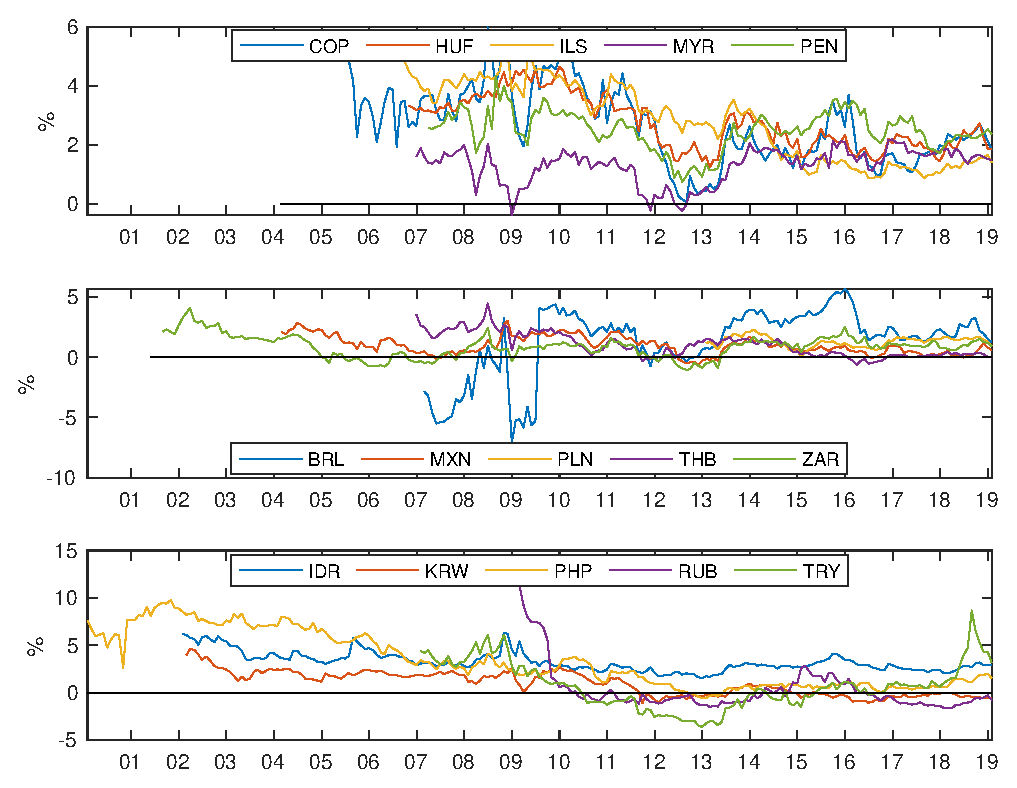
\includegraphics[trim={0 8.95cm 0 0}, clip, width=0.9\textwidth, height=0.65\textheight]{../Figures/Temp/temp_tp10yrEM}
			\par\end{center}
		\caption{Estimated 10-Year Term Premia.}\label{fig:tp_10yrA}
	\end{figure}
	\begin{textblock*}{3cm}(.97\textwidth,-.08\textheight)
		\hyperlink{tp_10yrB}{\beamergotobutton{B}}
	\end{textblock*}
\end{frame}
\note{EM TP are time-varying.}
\note{Sensible TP estimates, mostly positive; fluctuate between 0\% and 5\%.}
\note{Sometimes they comove.}


\begin{frame}
	\frametitle{Term Structure of Term Premia}
	\begin{figure}[!htbp]
		\begin{center}
			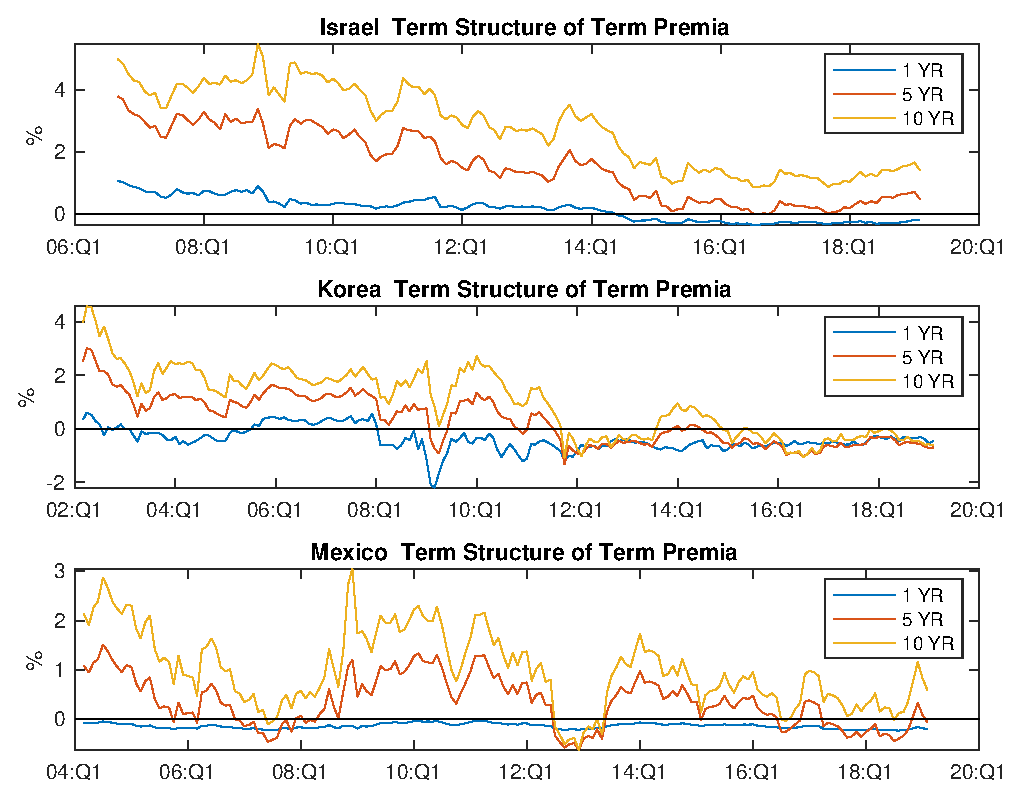
\includegraphics[trim={0 0 0 8.5cm}, clip, width=0.9\textwidth, height=0.65\textheight]{../Figures/Temp/temp_ts_tp}
			\par\end{center}
		\caption{Estimated 1-, 5- and 10-Year Term Premia.}\label{fig:tp_ts}
	\end{figure}
\end{frame}
\note{One can not only compare the TP across country but across maturities.}
\note{TP increases with maturity. As one would expect when LT are seen as risky, LT requiring a higher compensation.}
\note{Sometimes, standard deviation of TP increases with maturity.}

\begin{frame}
	\frametitle{Nominal Yield Curve Decomposition}
	\begin{tiny}\begin{table}\centering\begin{tabular}{l|ccccc}\toprule & Nominal & Synthetic & Expected & Term Premium & CIP Dev \\\midrule EM & 7.10 & 6.11 & 4.29 & 1.74 & 0.85 \\A-SOE & 3.48 & 3.52 & 1.54 & 1.97 & -0.23 \\G-3 & 2.41 & 2.13 & 0.52 & 1.60 & 0.15 \\\bottomrule\end{tabular}\caption{10-Year Yield Decomposition (\%).}\label{tab:decomp10yr}\end{table}\end{tiny}
	\begin{itemize}
		\item Estimated TP is higher on average than CIP deviations
		\item Main component of the nominal yield curve:
		\begin{itemize}
			\item For EMs, the expectation of the future short-term interest rate
			\item For AEs, the term premium
		\end{itemize}
	\end{itemize}
\end{frame}
\note{Deviations from CIP (CIP Dev) referred to as the LC credit spread (LCCS) for EMs and the convenience yield for AEs.}
\note{The dyanmics of TP and LCCS play an important role in EM bond yields.}
\note{It would be interesting to further decompose the nominal parts (Expected and TP) into real and inflation!!!}

\begin{frame}
	\frametitle{Term Premia: Does It Matter Which Curve Is Used?}
	\begin{tiny}\begin{table}\centering\begin{tabular}{l|cc}\toprule & Nominal & Synthetic \\\midrule EM & 2.17 & 1.74 \\A-SOE & 2.03 & 1.97 \\G-3 & 1.70 & 1.60 \\\bottomrule\end{tabular}\caption{10-Year Term Premium Comparison (\%).}\label{tab:tp_compare10yr}\end{table}\end{tiny}
	\begin{itemize}
		\item Difference between the two TP estimates is larger for EMs on average
		\begin{itemize}
			\item Null of equal means is rejected at $5$\% for 13 EMs vs 4 AEs
			\item For EMs, risk premium $\neq$ term premium
		\end{itemize}
	\end{itemize}
\end{frame}
\note{The null of equal means is rejected at the $5$\% significance level for all EMs except Hungary and Malaysia. However, the null is only rejected for four AEs (Australia, Denmark, Japan and New Zealand).}

\begin{frame}
	\frametitle{Is There A Global Factor in EM Term Premia?}
	\begin{tiny}\begin{table}\centering\begin{tabular}{l|cc}\toprule & Dec-2006 \\\midrule EM & 81.01 \\AE & 98.07 \\\bottomrule\end{tabular}\caption{Total Variation Explained by First 3 PCs (\%): 10-Year Term Premium.}\label{tab:temp_tp_common}\end{table}\end{tiny}
	\begin{itemize}
		\item Global financial cycle: Common factors on capital flows \citep{Rey:2013}
		\item For AEs, a global factor seems more relevant for TP
		\item For EMs, both domestic and global factors appear more relevant for TP
	\end{itemize}
\end{frame}

\begin{frame}
	\frametitle{Relationship with Risk and Uncertainty Measures}
	\begin{itemize}
		\item Comparison with US term premium
		\begin{itemize}
			\item TP
			\item $\perp$TP
		\end{itemize}
		\item CIP deviations: 
		\begin{itemize}
			\item LC credit spread \citep{DuSchreger:2016a}
			\item Convenience yield \citep{DuImSchreger:2018}
		\end{itemize}
		\item Uncertainty indexes \citep{BakerBloomDavis:2016}
	\end{itemize}
\end{frame}
\note{EPU index is based on frequency of key words -economy, uncertainty, Fed- in newspapers. Only available for 5 countries in the sample.}

\begin{frame}[label=corr_10yr]
	\begin{tiny}\begin{table}
		\centering
		\begin{tabular}{l|ccc}
			\toprule
			 & TP-USTP & TP-CIP Dev
			\\\midrule 
			EM & 0.60 & -0.28 \\
			A-SOE & 0.80 & -0.01 \\
			G-3 & 0.71 & -0.29 \\
			\bottomrule
		\end{tabular}
		\caption{Correlations of 10-Year Term Premia: U.S TP and CIP deviations}\label{tab:temp_tp_corr10yr}\end{table}\end{tiny}
	\begin{tiny}\begin{table}
		\centering
		\begin{tabular}{l|ccccc}
			\toprule
			 & BRL & COP & KRW & MXN & RUB \\
			 \midrule 
			 TP-EPU & 0.14 & 0.46 & -0.32 & 0.40 & -0.22 \\
%			 $\perp$TP-EPU & 0.11 & 0.28 & -0.31 & 0.20 & -0.09 \\
			 \bottomrule
		 \end{tabular}
	 \caption{Correlations of 10-Year Term Premia: Economic Policy Uncertainty Index}\label{tab:temp_tp_corr10yr_epu}\end{table}\end{tiny}
\end{frame}
\note{EM TP and US TP are closely related, it tends to increase with maturity.}
\note{Correlation with LCCS is negative. Possible explanation: LCCS low reaction to global variables while the TP's is high.}
\note{For EPU, need to study KRW and RUB more closely.}

\begin{frame}
	\frametitle{Drivers of EM Term Premia}
	\begin{itemize}
		\item Panel regressions per maturity
		%\vspace{-1cm}
		\begin{equation*} \label{eq:panelTPreg_nn}
	\eqpanelTPreg
\end{equation*}
		\vspace{-0.5cm}
		\begin{itemize}
			\item $tp_{it}$: model-based $\tnr$-year term premium of country $i$ in month $t$
			\item $z_{it}$: vector of regressors
			\item $\alpha_{i}$: country fixed effects
		\end{itemize}
	\end{itemize}
\end{frame}

\begin{frame}
\frametitle{Drivers of EM Term Premia: Regressors}
\begin{itemize}
	\item Global financial variables
	\begin{itemize}
		\item (log) VIX, fed funds rate (FFR), S\&P, oil price
	\end{itemize}
	\item Domestic variables
	\begin{itemize}
		\item Macro: Inflation, unemployment rate, industrial production
		\item Financial: exchange rate (LC per USD), stock market
	\end{itemize}
\end{itemize}
\end{frame}

\begin{frame}[label=pnl_tp10yr]
	\frametitle{10Y EM TP}
	\begin{center}
		\vspace{-1.1cm}
		\begin{tiny}
\begin{table}
\begin{center}
\begin{tabular}{lr@{\extracolsep{0pt}.}lr@{\extracolsep{0pt}.}l}
	%DEP. VARIABLE & \multicolumn{4}{l}{10Y EM TP}\tabularnewline
	& \multicolumn{2}{c}{(1)} & \multicolumn{2}{c}{(2)}\tabularnewline
	\hline 
	FFR & 0&11 & 0&923{*}{*}\tabularnewline
	& (0&10) & (0&355)\tabularnewline
	USTP10 & 1&22{*}{*}{*} & 0&521{*}{*}\tabularnewline
	& (0&16) & (0&237)\tabularnewline
	INF & 0&21{*}{*}{*} & 0&222{*}{*}{*}\tabularnewline
	& (0&05) & (0&040)\tabularnewline
	UNE & 0&13{*}{*} & 0&137{*}{*}\tabularnewline
	& (0&05) & (0&058)\tabularnewline
	IP & -0&02{*} & -0&019{*}{*}\tabularnewline
	& (0&01) & (0&008)\tabularnewline
	RFX & 0&01 & 0&0199{*}\tabularnewline
	& (0&01) & (0&0103)\tabularnewline
	Observations & \multicolumn{2}{c}{1,969} & \multicolumn{2}{c}{1,969}\tabularnewline
	R-squared & 0&49 & 0&547\tabularnewline
	Country FE & \multicolumn{2}{c}{Yes} & \multicolumn{2}{c}{Yes}\tabularnewline
	Time FE & \multicolumn{2}{c}{No} & \multicolumn{2}{c}{Yes}\tabularnewline
	\hline 
	\multicolumn{5}{l}{Robust standard errors in parentheses.}\tabularnewline
	\multicolumn{5}{l}{{*}{*}{*} p$<$0.01, {*}{*} p$<$0.05, {*} p$<$0.1}\tabularnewline
\end{tabular}%\caption{Panel Data Regressions of the 10-Year Term Premium (\%).} 
\label{tab:temp_tp_regs_slides}
\end{center}
\end{table}
\end{tiny}

 \par
	\end{center}
%	\begin{columns}
%		\begin{column}{0.3\textwidth}
%			%\large \textcolor{yaleblue}{\enskip 10Y EM TP}
%			\vfill
%		\end{column}
%		\begin{column}{0.7\textwidth}  %%<--- here
%			\begin{center}
%				\vspace{-1cm}
%					\begin{tiny}
\begin{table}
\begin{center}
\begin{tabular}{lr@{\extracolsep{0pt}.}lr@{\extracolsep{0pt}.}l}
	%DEP. VARIABLE & \multicolumn{4}{l}{10Y EM TP}\tabularnewline
	& \multicolumn{2}{c}{(1)} & \multicolumn{2}{c}{(2)}\tabularnewline
	\hline 
	FFR & 0&11 & 0&923{*}{*}\tabularnewline
	& (0&10) & (0&355)\tabularnewline
	USTP10 & 1&22{*}{*}{*} & 0&521{*}{*}\tabularnewline
	& (0&16) & (0&237)\tabularnewline
	INF & 0&21{*}{*}{*} & 0&222{*}{*}{*}\tabularnewline
	& (0&05) & (0&040)\tabularnewline
	UNE & 0&13{*}{*} & 0&137{*}{*}\tabularnewline
	& (0&05) & (0&058)\tabularnewline
	IP & -0&02{*} & -0&019{*}{*}\tabularnewline
	& (0&01) & (0&008)\tabularnewline
	RFX & 0&01 & 0&0199{*}\tabularnewline
	& (0&01) & (0&0103)\tabularnewline
	Observations & \multicolumn{2}{c}{1,969} & \multicolumn{2}{c}{1,969}\tabularnewline
	R-squared & 0&49 & 0&547\tabularnewline
	Country FE & \multicolumn{2}{c}{Yes} & \multicolumn{2}{c}{Yes}\tabularnewline
	Time FE & \multicolumn{2}{c}{No} & \multicolumn{2}{c}{Yes}\tabularnewline
	\hline 
	\multicolumn{5}{l}{Robust standard errors in parentheses.}\tabularnewline
	\multicolumn{5}{l}{{*}{*}{*} p$<$0.01, {*}{*} p$<$0.05, {*} p$<$0.1}\tabularnewline
\end{tabular}%\caption{Panel Data Regressions of the 10-Year Term Premium (\%).} 
\label{tab:temp_tp_regs_slides}
\end{center}
\end{table}
\end{tiny}

 \par
%			\end{center}
%		\end{column}
%	\end{columns}
	
	
%	\begin{textblock*}{3cm}(.92\textwidth,-.955\textheight)
%		\hyperlink{pnl_tp5yr}{\beamergotobutton{5YR}}
%	\end{textblock*}
\end{frame}
\note{Main broad message at 10 years. Big difference: FFR more negative when there is no USTP and disappears when USTP}
\note{Country fixed-effects were included to allow for the possibility that country-specific factors that may affect TP are also correlated with the controls.}
\note{External conditions have a relevant impact on domestic bond markets. }
\note{The channel does not seem to be through the VIX nor even through the monetary policy of the U.S. directly via the federal funds rate but through the U.S. term premia.}
\note{The effect of the domestic variables is in line with what has been found for AEs. 
	Investors demand a higher term premium during recessions, when the unemployment rate increases. This shows evidence of a countercyclical behavior of the TP in EMs.
	The positive effect of inflation on the TP conforms with the idea that inflation erodes the value of nominal bonds and so in periods of rising inflation investors demand a higher TP.}
\note{A depreciation of the LC is associated with an increase in the TP. This seems counterintuitive since EMs are usually commodity exporters so it appears to contradict the standard trade-channel effect. However, it is in line with the risk-taking channel of exchange rates found by \cite{HofmannShimShin:2017}, according to which currency appreciation is associated with easier financial conditions and compressed sovereign bond spreads.}

\begin{frame}
	\frametitle{Work in Progress}
	\begin{itemize}
		\item Survey forecasts so far as a robustness check. Next: supplement ATSM
		\item Controls to include when studying the drivers of TP:
		\begin{itemize}
			\item Measures of inflation uncertainty (Stock and Watson, 2007)
			\item Measures of political uncertainty \citep{BakerBloomDavis:2016}
		\end{itemize}
	\item How U.S. monetary policy moves EM yields?
	\begin{itemize}
		\item Event study methodology (G\"{u}rkaynak and Wright, 2013)
		\item Local projections (Jord\`a, 2005)
	\end{itemize}
	\end{itemize}
\end{frame}
\note{There is clearly uncertainty in the TP estimates and that is where survey forecasts can be helpful.}


\section{Conclusions}

\begin{frame}
	\frametitle{Conclusions}
	\begin{itemize}
		\item `Clean' EM TP estimates using synthetic LC yield curves
		\begin{itemize}
			\item Gains from `adjusting' for credit risk
			\item In EMs, risk premium $\neq$ term premium
			\item More disaggregated decomposition of nominal LC yield curves
		\end{itemize}
		\item Properties of EM term premia
		\item Several potential extensions
	\end{itemize}
\end{frame}
\note{Potential extensions: nominal and real decompositions, multi-country models, models with jumps.}

\section{Internship}

\begin{frame}
\begin{center}
	\huge \textcolor{yaleblue}{Internship Proposals}
\end{center}
\end{frame}

\begin{frame}
	\frametitle{Proposals}
	\begin{itemize}
		\item Effects of changes in the yield curve on the banking system
		\item Effects of monetary policy on the banking system
		\begin{itemize}
			\item Whose monetary policy?
			\begin{itemize}
				\item Mexico vs U.S.
			\end{itemize}
			\item Effects on what?
			\begin{itemize}
				\item Prices: bank stock returns, deposit rates
				\item Quantities: size of deposits, loans, balance sheet
				\item Performance: interest rate risk, NIM, ROA, ROE
			\end{itemize}
		\end{itemize}
	\end{itemize}
\end{frame}
\note{Altavilla et al. (2018): Banks' profits are crucial for banks' capital and hence for financial stability.}
\note{Stock market returns provide market-based expectations on future profitability.}

\begin{frame}
	\frametitle{Proposal 1}
	\begin{itemize}
		\item Challenge of assessing impact of MP: Isolate exogenous policy changes
		\item Identification of monetary policy shocks
		\begin{itemize}
			\item SVAR for quarterly data and macro variables (e.g. GDP, inflation, policy rate)
			\item Ordering is not straight forward when using other financial variables
		\end{itemize}
		\item In such cases, high-frequency event studies allow for identification
		\begin{itemize}
			\item Changes in interest rate futures contracts around MP announcements
			\item But tool rely on federal funds futures rates $\rightarrow$ U.S. specific
		\end{itemize}
	\end{itemize}
\end{frame}
\note{G\&W (2013): As both MP and asset prices are forward-looking, they react to each other within the quarter.}
\note{Altavilla et al. (2018): Changes in small windows around announcements, captures the efficient market reaction to new information and thus reflects the causal impact of MP.}
\note{Lloyd (208): FFFs are US-specific and very few similar instruments are traded elsewhere.}
\note{Banxico don't have access to historical HF data.}

\begin{frame}
	\frametitle{Proposal 1}
	\begin{itemize}
	\item \textbf{Proposal}: Are there real effects of HF-identified U.S. MP shocks on local credit conditions?
	\begin{itemize}
		\item Quantities: size of deposits, loans, bank balance sheets
	\end{itemize}
	\item Evidence on the international bank-lending channel using Mexican data
	\begin{itemize}
		\item Morais, Peydró, Roldán-Peña and Ruiz (2019)
		\item But they don't identify U.S. MP shocks using HF data
	\end{itemize}
	\end{itemize}
\end{frame}

\begin{frame}
	\frametitle{Proposal 2}
	\begin{itemize}
		\item Theoretically, effects of expansionary MP on bank performance are ambiguous
		\begin{itemize}
			\item Higher present value of future cash flows $\rightarrow$ Higher stock price
			\item Lower net interest margin $\rightarrow$ Lower ROA
		\end{itemize}
		\item Mixed evidence on the effects of MP on bank performance
		\begin{itemize}
			\item Negative effect ($-$): English et al. (2018)
			\item Positive effect ($+$): Claessens et al. (2018)
			\item Reversal effect ($-$, $+$): Ampudia and Van den Heuvel (2018), Yuan (2019)
			\item No effect: Altavilla et al. (2018), Drechsler et al. (2018)
		\end{itemize}
	\end{itemize}
\end{frame}
\note{Drawback with HF MP shocks: persistency of effect.}
\note{Altavilla et al. (2018): Net effect of MP on bank profitability is an empirical question.}
\note{Even among those that find no effect, they differ. Altavilla et al. (2018) no overall effect because effect on ROA components offset, while Drechsler et al. (2018) no effect because ROA components insensitive to changes in interest rates.}
\note{Topic has attracted a lot of attention recently due to concerns on the potential side effects for banks of very low interest rates in AEs.}

\begin{frame}
	\frametitle{Proposal 2}
	\begin{itemize}
		\item \textbf{Proposal}: Effects of MXN monetary policy changes on banks' performance
		\begin{itemize}
			\item Interest rate risk, NIM, ROA
		\end{itemize}
		\item Main implication of no effect $\rightarrow$ Deposits channel of MP not limited to AEs
		\begin{itemize}
			\item Banks unexposed to interest rate risk
			\begin{itemize}
				\item Market power over deposits lowers sensitivity of banks' expenses
			\end{itemize}
			\item Maturity transformation \textit{hedges} banks' interest rate risk
			\begin{itemize}
				\item Banks invest in long-term assets to hedge their deposit franchise
			\end{itemize}
		\end{itemize}
		\item DC might be behind both: bank-lending and risk-taking channels of MP
	\end{itemize}
\end{frame}
\note{Old view: perfect competition in deposit side. New view: imperfect competition on deposit side.}
\note{DC: MP not only affects loan supply but also deposit supply.}
\note{By affecting the deposit supply, MP influences loan supply and credit spreads (appetite for risk).}

\begin{frame}
	\frametitle{Data Needed}
	\begin{itemize}
		\item EM TP: Surveys from Consensus Economics for Latam countries since 2013
		\item Proposal 1: Quantities
		\begin{itemize}
			\item Size of deposits, loans, bank balance sheets
		\end{itemize}
		\item Proposal 2: Interest expense and interest income over assets. Plus:
		\begin{itemize}
			\item Deposit rates, durations of assets and liabilities
		\end{itemize}
		\item P1 \& P2: NIM, ROA
	\end{itemize}
\end{frame}

\section{Appendix}

\begin{frame}
	\begin{center}
		\huge \textcolor{yaleblue}{Appendix}
	\end{center}
\end{frame}

\begin{frame}[label=tp_10yrB]
	\frametitle{EM Term Premium Estimates: 10Y (cont.)}
	\begin{figure}[!htbp]
		\begin{center} % trim removes: left, down, right, top
			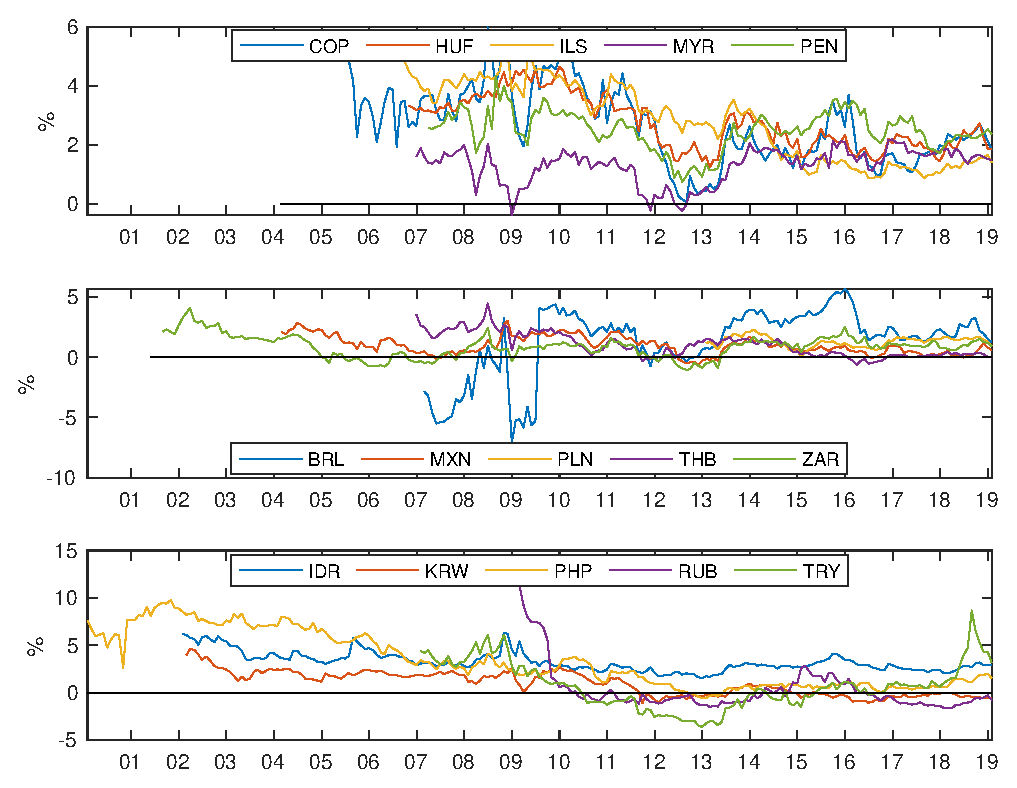
\includegraphics[trim={0 0 0 4cm},clip, width=0.9\textwidth,height=0.65\textheight]{../Figures/Temp/temp_tp10yrEM}
			\par\end{center}
		%\caption{Estimated 10-Year Term Premia (cont.).}\label{fig:tp_10yrB}
	\end{figure}
	\begin{textblock*}{3cm}(.97\textwidth,-.08\textheight)
		\hyperlink{tp_10yrA}{\beamerreturnbutton{A}}
	\end{textblock*}
\end{frame}

\begin{frame}
	\frametitle{Survey-Based Term Premium Estimates}
		\begin{figure}[!htbp]
		\begin{centering}
			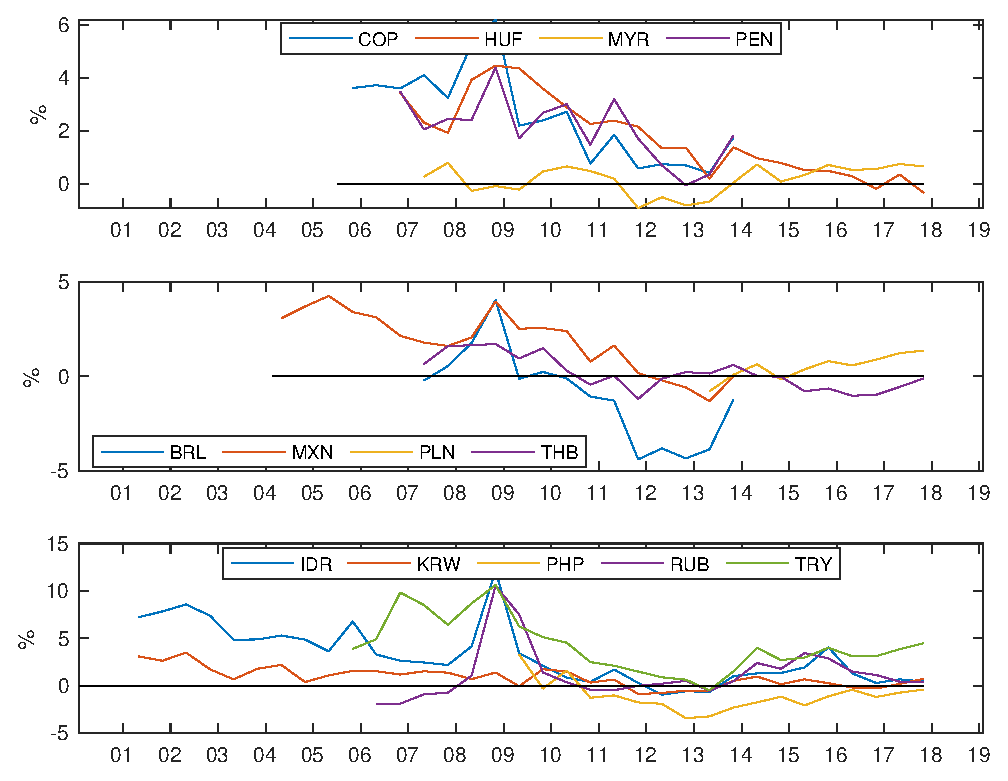
\includegraphics[width=1\textwidth,height=0.5\textheight]{../Figures/Temp/temp_tp10yrSvy}
			\par\end{centering}
		\caption{Survey-Based 10-Year Term Premium Estimates}\label{fig:temp_tp10yrSvy}
	\end{figure}
%	\begin{textblock*}{3cm}(.97\textwidth,-.08\textheight)
%		\hyperlink{tp_10yrA}{\beamerreturnbutton{A}}
%	\end{textblock*}
\end{frame}


\begin{frame}<presentation:0>
\bibliographystyle{abbrvnat} 
\bibliography{../../../References/library}
\end{frame}

\end{document}

%---------------------------------------------------------------
% Sources
%---------------------------------------------------------------
% Tips in general
% https://en.wikibooks.org/wiki/LaTeX/Presentations
%https://tex.stackexchange.com/questions/12328/how-can-i-use-todonotes-with-beamer
% Insert links to slides
% https://latex.org/forum/viewtopic.php?t=4594
% Place button of link on slide
%https://tex.stackexchange.com/questions/50643/hyperlink-button-in-an-exact-position
% Make figures visible
%https://stackoverflow.com/questions/4683093/beamer-how-to-show-images-as-step-by-step-images
% Multicolumn and multirow
%https://tex.stackexchange.com/questions/156219/proper-centering-with-cmidrule-and-multi-row-and-column

% Code for hyperlinks
%[label=corr_10yr]
%\begin{textblock*}{3cm}(.9\textwidth,-.5\textheight)
%	\hyperlink{corr_10yr}{\beamergotobutton{10-Year TP}}
%\end{textblock*}
%
%\begin{textblock*}{3cm}(.9\textwidth,-.5\textheight)
%	\hyperlink{corr_10yr}{\beamerreturnbutton{10-Year TP}}
%\end{textblock*}

% Two-column frame template
%http://felix11h.github.io/blog/beamer-two-col